%\begin{document}
\documentclass[a4paper,12pt]{article}
\usepackage{indentfirst}%paragrafo no primeiro tb
\usepackage[english,brazil]{babel}
\usepackage[utf8]{inputenc}
\usepackage{amsmath}
\usepackage{graphicx}
\usepackage{fancyhdr}
\usepackage{url}
\renewcommand{\baselinestretch}{1.5}
\usepackage{setspace}%%%% pacote para espaço duplo
\usepackage{titling}
\usepackage{geometry}
\usepackage{amsmath}
\usepackage{amssymb}
%\usepackage{subfigure}
\usepackage{multirow}
\usepackage[table]{xcolor}
\usepackage{fullpage}
\usepackage[backend=bibtex,style=ieee,sorting=none]{biblatex}
\usepackage{subfig}
\bibliography{refs}


\newcolumntype{C}{>{\centering\arraybackslash}p{1em}}

% FAPESP pede "tipo equivalente a Times New Roman"
% Acho que na verdade eles só estão preocupados com o tamanho da fonte
% A diferença entre a fonte padrão do LaTeX e times é pequena
%\usepackage{times}

\title{\textbf{Controle de Estabilização de Caminhada de Robô Humanoide
}\\
\vspace{30px}
\normalsize \textbf{Projeto de Pesquisa para Iniciação Científica}\\
 \textbf{Laboratório de Sistemas Computacionais Autônomos}\\
 \textbf{Instituto Tecnológico de Aeronáutica -- ITA}
 }






%%%%


\author{\textbf{Beneficiário:} Reynaldo Santos de Lima\\
\textbf{Orientador:} Marcos Ricardo Omena de Albuquerque Maximo\\
 } %\\

%%%%%%%

\date{\today}
% ADD THE FOLLOWING COUPLE LINES INTO YOUR PREAMBLE
\let\OLDthebibliography\thebibliography
\renewcommand\thebibliography[1]{
  \OLDthebibliography{#1}
  \setlength{\parskip}{0pt}
  \setlength{\itemsep}{0pt plus 0.3ex}
}


\begin{document}
\maketitle

%\newpage
%\maketitle


%\thispagestyle{empty}
\begin{abstract}
Neste trabalho pretende-se aplicar adaptações em algoritmos de estabilização de caminhada em robô humanoide de baixo custo (ITAndroids Chape 1ª e 2ª gerações). Esse trabalho será realizado no  Laboratório de Sistemas Computacionais Autônomos (LAB-SCA), onde  existe um estudo de caminhada de robôs humanoide, Robotis OP2 e ITAndroids Chape. O controle utilizado para o desenvolvimento da caminhada já presente no robô Chape 1ª geração será estudado numa primeira etapa. Este se baseia no método \textit{Preview Control of Zero-Moment Point}, ZMP. O código já utilizado será estudado com o objetivo de encontrar possíveis otimizações como também de adaptá-lo para o robô Chape 2ª geração.

Utilizar-se-á do simulador Gazebo, já utilizado em trabalhos realizados no LAB-SCA, para validar a estabilização implementada e os ajustes de desempenho empregados. Com a validação no simulador, pretende-se realizar ensaios com o robô real, verificando a efetividade do trabalho desenvolvido com o auxílio de unidade inercial embarcada dos robôs.


\noindent \textbf{Palavras chaves:} Caminhada de robôs humanoides, Controle, Robótica.


%%%
\end{abstract}
\selectlanguage{english}

\title{\textbf{Control for Humanoid Walking Stabilization
}\\
\vspace{30px}
\normalsize \textbf{Scientific Initiation Project}\\
 \textbf{Autonomous Computational Systems Laboratory}\\
 \textbf{Aeronautics Institute of Technology -- ITA}
 }






%%%%


\author{\textbf{Beneficiary:} Reynaldo Santos de Lima\\
\textbf{Advisor:} Marcos Ricardo Omena de Albuquerque Maximo\\
 } %\\
 
\maketitle 
 
\begin{abstract}
In this work, we intend to apply adaptations in algorithms for humanoid robot walking stabilization in low-cost humanoid robots (ITAndroids Chape 1st and 2nd generations). This work will take place in the Autonomous Computational Systems Lab (LAB-SCA), where there is a study of humanoid robot walking, Robotis OP2 and ITAndroids Chape. The control technique used for the development of the current walking in the Chape 1st generation robot will be studied in a first phase. This is based on the method of Preview Control of Zero-Moment Point, ZMP. The developed code will also be studied with the goal of possible optimizations as well as to adapt it to the Chape 2nd generation robot.

We will use the Gazebo simulator, which is already used in works done in LAB-SCA, to validate the implemented stabilization controller and the employed performance adjustments. After the validation in the simulator, we intend to execute experiments with the real robot, verifying the effectivity of the developed work with the use of the inertial measurement unit embedded in the robots.

\noindent \textbf{Keywords:} Humanoid robot walking, Control, Robotics.


%%%
\end{abstract}
%%%
\selectlanguage{brazil}
%%%%%
\doublespacing
\newpage
%%%%%%
\section{Introdução, Justificativa e Síntese da Bibliografia Fundamental}
%\label{secao:enunciado_problema}



No contexto da robótica móvel existem diversos problemas a serem abordados e um que se destaca é o estudo de robôs humanoides, especificamente a questão da caminhada. O estudo de robôs humanoides tem motivação na movimentação de robôs por terrenos irregulares, destacando-se que os ambientes desenvolvidos pelo homem são propícios para bípedes. Desse modo, por mais que o controle de robôs com rodas seja mais simples e demonstrem alta eficência, o movimento é limitado a terrenos planos, sendo uma solução para o problema a caminhada de robôs com pernas.

Dos movimentos de robôs com pernas, o movimento bípede do humanoide é de fundamental interesse exatamente pela proximidade ao movimento do ser humano. Esse movimento é uma ação complexa do ponto de vista de controle, devido às não linearidades, a subatuação e  de envolver uma dinâmica com alta dimensionalidade, ou seja, muitos graus de liberdade. Representando um grande desafio às técnicas de controle de última geração \cite{tedrake2005}.

Uma primeira questão a ser analisada é a estabilidade estática dos bípedes é assegurada pela projeção de centro de massa (CM) no solo dentro de um polígono de suporte, definido na Literatura como a envoltória convexa dos pontos de contato no solo. Consequentemente, na estática, as forças de reação do solo atuam na vertical no ponto que equivale à projeção do CM para equilibrar as forças e momentos gerados pela gravidade, sendo o centro de pressão (CP) o ponto resultante das forças de reação.

Para desenvolver uma caminhada estável e rápida em robôs bípedes é necessário considerar os efeitos dinâmicos sobre o CP. Um conceito popular nesse contexto  utilizado é o Zero Moment Point (ZMP), que pode ser encarado  como o ponto no solo onde as forças de reação devem atuar para estabilizar o mecanismo bípede \cite{vukobratovic2004} assim, quando o ZMP estiver dentro do polígono de suporte, este coincide com o CP.

Quando em regime dinâmico o CM e o CP não coincidem, mas a aceleração do corpo auxilia na obtenção do equilíbrio. Por isso, na prática, para preservar a estabilidade basta delinear o movimento de maneira que o ZMP esteja sempre dentro do polígono de suporte. Na marcha há sempre um pé em contato com o solo em algum momento da caminhada e isso auxilia na transição para o apoio seguinte.

Como robôs humanoides têm muitos graus de liberdade e sua dinâmica é não linear, o movimento se torna complexo. Por isso, geralmente são usados modelos de ordem reduzida.  Por exemplo, com o 3D Linear Inverted Pendulum Model (3D-LIPM)\cite{kajita2001}, pode-se obter a trajetória do CM e depois, por cinemática inversa, determinar os ângulos das juntas durante a caminhada. Por causa das simplificações do modelo, frequentemente usam-se estratégias de realimentação e compensação de erro de dinâmica para o robô ter estabilidade \cite{yoshiike2009}.


Por outro lado, os critérios exigidos na modelagem da caminhada de humanoide são altamente restritivos quanto à estabilidade. Os critérios utilizados mais corriqueiramente tratam da estabilidade local da caminhada, isto é, observa-se as condições de estabilidade para o estado atual do robô a cada passo, não para a caminhada como um todo. O ZMP, por exemplo, trata-se de um critério que observa apenas a estabilidade local.

O fato da análise de estabilidade ser tratada localmente tornam os critérios estabelecidos restritivos, produzindo um movimento de caminhada muito aquém do melhor movimento quanto ao aproveitamento energético. Para comparação, estima-se que o robô ASIMO utiliza 10 vezes mais energia que um ser humano para caminhar. \cite{tedrake2005}.

Existem outros critérios mais gerais, como o ``caminhada em ciclo limite'', \cite{inbook} que estabelecem movimentos instáveis a cada passo mas estáveis num ciclo completo de caminhada. Isto é, o ZMP deixa o polígono de suporte, acelerações angulares são geradas, mas movimentos posteriores a esse momento instável permitem que a caminhada continue. Este tipo de movimento exige uma análise de todo o percurso a ser tomado, tornando a execução pouco praticável.

Com as limitações expostas e ao observar os resultados obtidos com sucesso na prática \cite{tedrake2005}, caminhadas baseadas no critério ZMP mostram-se como estado-da-arte, sendo o critério escolhido para estabilização de caminhada.


O grupo de pesquisa do Laboratório de Sistemas Computacionais Autônomos (LAB-SCA) do ITA tem desenvolvido estudos na área de caminhada de robôs humanoides\cite{max22,max25,max27,max28,tesemarcos}.
No trabalho mais recente \cite{tesemarcos}, investigaram-se formulações baseadas em  Controle Preditivo  que permitem ao robô decidir a 
trajetória do CM, as posições dos pés e durações dos passos \cite{7759794}.

Na figura \ref{FIG:darwinchape} (a) pode ser visto um robô humanoide Robotis OP2 com o qual o grupo iniciou seus estudos em caminhada; na Figura \ref{FIG:darwinchape} (b) observa-se o robô ITAndroids Chape 1ª geração, robô humanoide desenvolvido pelo LAB-SCA. O desempenho dos robôs utilizados no LAB-SCA tem se mostrado como referência nacional em competições de robótica, campeão do futebol de robôs humanoide em 2018 e 2019 na Latin American Robotics Competition (LARC). Com os trabalhos desenvolvidos, faz-se essencial o desenvolvimento contínuo do projeto das malhas de controle de estabilização de caminhada.

\begin{figure}[phtb]
\centering
	\centering
    \subfloat[]{{\includegraphics[width=0.2483\textwidth]{darwin.jpg}}}
    	\subfloat[]{{\includegraphics[width=0.25\textwidth]{chape.jpg}}}
\caption{Modelo de robôs humanóides do LAB-SCA, a) Robotis OP2 b) Chape.}
\label{FIG:darwinchape}
\end{figure}

De modo geral, o movimento periódico da caminhada é resolvido em termos de controle com uma sequência de algoritmos que formam uma malha de controle fechada. Uma visão geral da arquitetura da malha de controle pode ser vista na Figura \ref{FIG: doc manga}. Tem-se como entrada um vetor de velocidade omnidirecional desejado, para ser gerado no planejador de passos as posições e tempos da marcha. Com o planejamento definido, utiliza-se um algoritmo gerador de trajetórias baseado na posição do ZMP de acordo com o pé de apoio (Gerador de Trajetórias ZMP, na Figura \ref{FIG: doc manga}). Planeja-se ainda a trajetória do CM (com retorno de sensores sobre posição, velocidade e aceleração para o controle) e do pé de balanço, aquele não em contato com o solo no passo, a fim de definir totalmente as trajetórias a serem cumpridas.

Solucionado o movimento desejado, entra o algoritmo Solucionador de Cinemática Inversa, que calcula as posições necessárias das juntas para que os pés fiquem na posição desejada. Além de resolver a cinemática, fazem-se necessários ainda dois passos na malha de controle, representados pelo compensador de gravidade e pelo compensador de orientação do torso.

A necessidade do compensador de gravidade surge da atuação de torques indesejados nas juntas do robô causados pela aceleração da gravidade e é implementado em momentos de suporte único no passo (isto é, quando o robô tem uma perna suporte e outra livre de contato com o solo) e de suporte duplo (considerando este uma combinação das soluções para as pernas direita e esquerda consideradas, para cada solução, como único pé de suporte). Já o compensador de orientação do torso surge principalmente para compensar erros de medidas ou de perturbações externas. Este é implementado com uma malha de controle P+V. O algoritmo para o compensador de orientação de torso, por sua vez, observa a posição do torso em cada passo utilizando Filtro de Kalman Estendido (EKF) para o tratamento dos dados oriundos dos sensores \cite{tesemarcos}.
 
\begin{figure} 
	\centering
	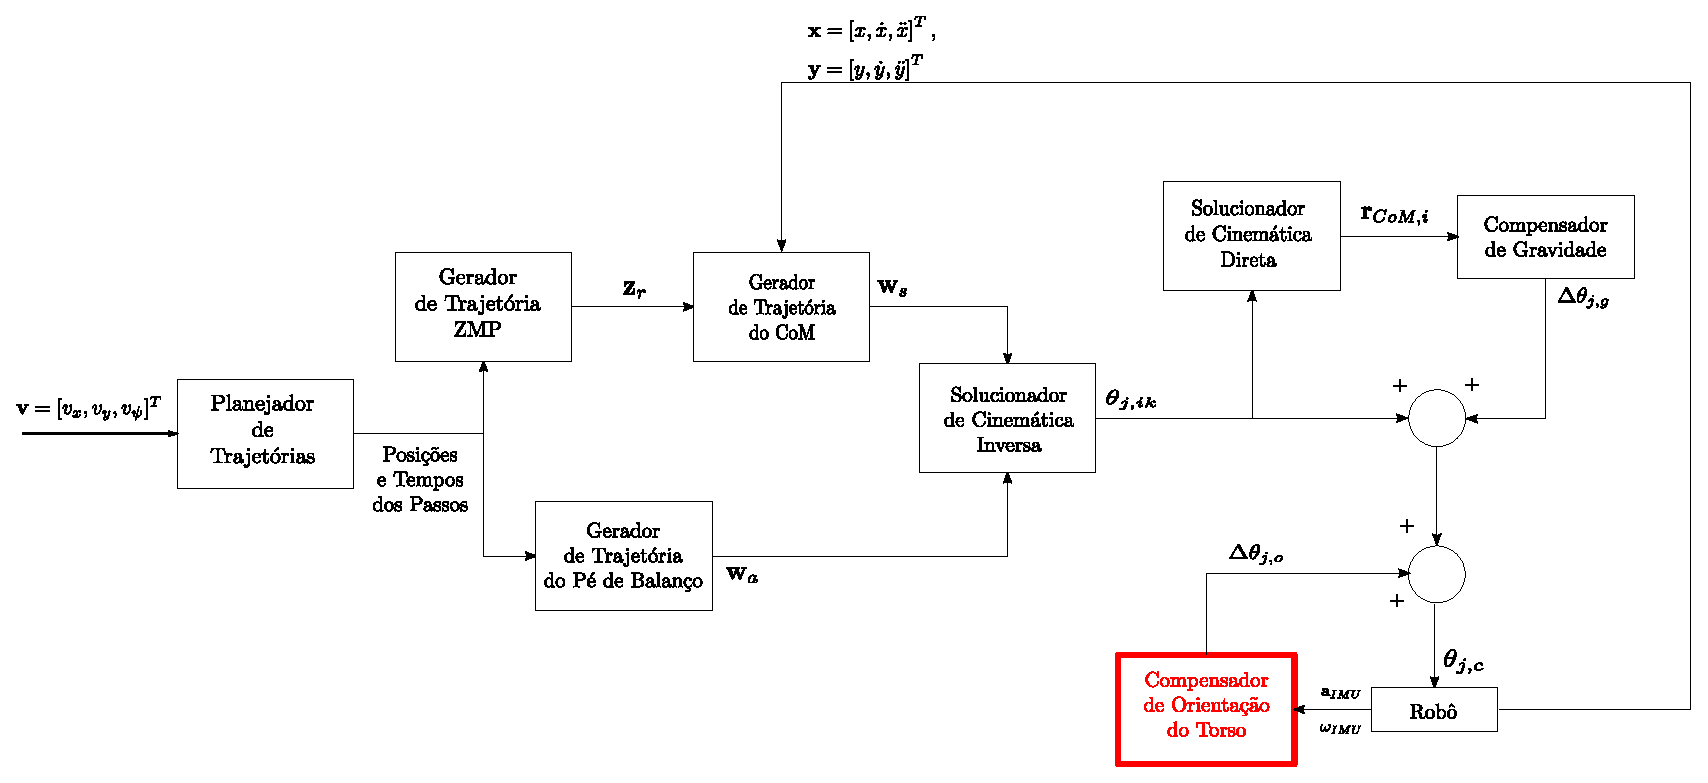
\includegraphics[angle=90, scale = 0.75]{walking_engine_overview.eps}
	\caption{Visão geral do controle de caminhada.}
	\label{FIG: doc manga}
\end{figure} 
 

O embasamamento matemático dos métodos propostos será apresentado a seguir:


\subsection{Preview Control of ZMP}

O \emph{Preview Control of Zero-Moment Point} é um método de controle de caminhada bípede baseado em Controle Preditivo Baseado em Modelo (\emph{Model Predictive Control} -- MPC) \cite{kajita2003}. Não apenas esse método foi implementado em vários robôs humanoides \cite{yi2016}, mas  também serve de base para técnicas no estado da arte \cite{tesemarcos,herdt2010}. Além disso, o LAB-SCA tem experiência no uso desse tipo de algoritmo de caminhada \cite{max22,tesemarcos}, de modo que o \emph{Preview Control of ZMP} será um ponto de partida para esse trabalho. Nessa subseção, apresentar-se-á uma introdução teórica a esse método.

MPC é uma abordagem moderna de controle ótimo em que o comportamento futuro do sistema dinâmico é previsto através da integração de um modelo matemático. A inspiração para o uso de MPC advém do fato de que, durante a caminhada, mudanças instantâneas ocorrem no polígono de suporte devido aos pés do robô fazerem e quebrarem contato com o chão. Com isso, é interessante que o controlador de caminhada anticipe a referência futura de ZMP ao mover o ZMP antes que uma mudança repentina de polígono de suporte aconteça.

A seguir, deduz-se as equações apenas para o eixo de coordenadas \( x \), dado que estendê-las para o eixo \( y \) é trivial. Primeiramente, considere controle direto sobre a sobre-aceleração (i.e. derivada da aceleração) do CM do robô  \( \dddot{x} \), então a evolução temporal do CM é ditada por cinemática. Assumindo-se a hipótese de segurador de ordem zero sobre um passo de tempo de duração \( T \), pode-se obter o seguinte modelo de tempo discreto para a dinâmica do CM:
\begin{equation}
\mathrm{\mathbf{x}}[k+1] = \begin{bmatrix}
1 & T & T^2/2 \\ 0 & 1 & T \\ 0 & 0 & 1
\end{bmatrix} \mathrm{\mathbf{x}}[k] + \begin{bmatrix}
T^3/6 \\ T^2/2 \\ T
\end{bmatrix} \dddot{x}[k],
\label{eq:discrete_dynamics_x}
\end{equation}
em que \( \mathrm{\mathbf{x}}[k] = \left[ x[k] \ \dot{x}[k] \ \ddot{x}[k] \right]^T \). Além disso, se a altura do CM \( h \) é mantida constante e a variação do momento angular é ignorada, a dinâmica do ZMP segue o conhecido modelo de pêndulo invertido \cite{kajita2001}:
\begin{equation}
z_x[k] = \begin{bmatrix}
1 & 0 & -h/g
\end{bmatrix} \mathrm{\mathbf{x}}[k],
\label{eq:zmp}
\end{equation}
em que \( g \) é a aceleração da gravidade. A predição do comportamento futuro do sistema em um horizonte de \( N \) passos de tempo, dada uma sequência de comandos \( \dddot{\mathrm{\mathbf{X}}}[k] = \left[\dddot{x}[k|k] \ \cdots \ \dddot{x}[k+N-1|k] \right]^T \), pode ser obtida por:
\begin{equation}
\mathrm{\mathbf{X}}[k] = \begin{bmatrix}
x[k+1|k] \\
%x[k+2|k] \\
\vdots \\
x[k+N|k]
\end{bmatrix} = \mathrm{\mathbf{P}}_{ps} \mathrm{\mathbf{x}}[k] + \mathrm{\mathbf{P}}_{pu} \dddot{\mathrm{\mathbf{X}}}[k], \
\dot{\mathrm{\mathbf{X}}}[k] = \begin{bmatrix}
\dot{x}[k+1|k] \\
%\dot{x}[k+2|k] \\
\vdots \\
\dot{x}[k+N|k]
\end{bmatrix} = \mathrm{\mathbf{P}}_{vs} \mathrm{\mathbf{x}}[k] + \mathrm{\mathbf{P}}_{vu} \dddot{\mathrm{\mathbf{X}}}[k],
\label{eq:dx_pred}
\end{equation}
\begin{equation}
\ddot{\mathrm{\mathbf{X}}}[k] = \begin{bmatrix}
\ddot{x}[k+1|k] \\
%\dot{x}[k+2|k] \\
\vdots \\
\ddot{x}[k+N|k]
\end{bmatrix} = \mathrm{\mathbf{P}}_{as} \mathrm{\mathbf{x}}[k] + \mathrm{\mathbf{P}}_{au} \dddot{\mathrm{\mathbf{X}}}[k], \
\mathrm{\mathbf{Z}}_x[k] = \begin{bmatrix}
z_x[k+1|k] \\
%z_x[k+2|k] \\
\vdots \\
z_x[k+N|k]
\end{bmatrix} = 
\mathrm{\mathbf{P}}_{zs} \mathrm{\mathbf{x}}[k] + \mathrm{\mathbf{P}}_{zu} \dddot{\mathrm{\mathbf{X}}}[k],
\label{eq:zx_pred}
\end{equation}
em que as matrizes \( \mathrm{\mathbf{P}}_{ps} \), \( \mathrm{\mathbf{P}}_{pu} \), \( \mathrm{\mathbf{P}}_{vs} \), \( \mathrm{\mathbf{P}}_{vu} \), \( \mathrm{\mathbf{P}}_{as} \), \( \mathrm{\mathbf{P}}_{au} \), \( \mathrm{\mathbf{P}}_{zs} \), e \( \mathrm{\mathbf{P}}_{zu} \) podem ser determinadas usando as equações \eqref{eq:discrete_dynamics_x} e \eqref{eq:zmp}. Assim, rastreia-se uma trajetória futura de ZMP de referência sobre um horizonte através do uso da seguinte função de custo:
\begin{equation}
J \left( \dddot{\mathrm{\mathbf{X}}}[k] \right) = \frac{\alpha}{2} || \dddot{\mathrm{\mathbf{X}}}[k] ||^2 + \frac{\gamma}{2} || \mathrm{\mathbf{Z}}_{r,x}[k] - \mathrm{\mathbf{Z}}_x[k] ||^2,
\label{eq:optimization_preview}
\end{equation}
em que os pesos \( \alpha \) e \( \gamma \) penalizam o uso de sobre-aceleração e o erro de rastreio de ZMP, respectivamente. Além disso, \( \mathrm{\mathbf{Z}}_{r,x}[k] \) é a trajetória de referência de ZMP no eixo \( x \), i.e. \( \mathrm{\mathbf{Z}}_{r,x}[k] = \left[z_{r,x}[k+1] \ \cdots \ z_{r,x}[k+N] \right]^T \).

Para o máximo de estabilidade, o artigo original sugere escolher uma referência de ZMP poligonal que mantém o ZMP no meio do pé de suporte durante suporte simples e move o ZMP entre os pés durante suporte duplo \cite{kajita2003}. A hipótese implícita aqui é que o rastreio de ZMP é bom o suficiente para manter o ZMP sempre dentro do polígono de suporte, como exigido pelo critério de estabilidade de ZMP \cite{vukobratovic2004}. Porém, outro tipo de referência é mais interessante caso deseje-se reduzir consumo energético, conforme já explorado por pesquisadores do LAB-SCA \cite{max22}.

O algoritmo de \emph{Preview Control of ZMP} é usado em conjunto com um planejador de passos que escolhe as posições dos pés de acordo com um objetivo de alto nível. A trajetória de sobre-aceleração é obtida através da solução do problema de otimização definido pela função de custo \eqref{eq:optimization_preview}, o qual possui solução analítica:
\begin{equation}
\dddot{\mathrm{\mathbf{X}}}[k] = \left( \mathrm{\mathbf{P}}^T_{zu} \mathrm{\mathbf{P}}_{zu} + \frac{\alpha}{\gamma} \mathrm{\mathbf{I}}_N \right)^{-1} \mathrm{\mathbf{P}}^T_{zu} \left( \mathrm{\mathbf{Z}}_{r,x} - \mathrm{\mathbf{P}}_{zs} \mathrm{\mathbf{x}}[k] \right),
\end{equation}
em que \( \mathrm{\mathbf{I}}_N \) representa a matriz identidade de tamanho \( N \). Como não é possível controlar diretamente sobre-aceleração em um robô com atuadores de posição, como o Robotis OP2 ou o Chape, é necessário reconstruir a trajetória de CM usando \eqref{eq:dx_pred}. Para mais informações sobre como implementar essa técnica em um robô real, sugere-se ler \cite{tesemarcos}.

Um ponto que se deve destacar é que esse método se baseia no consagrado 3D-LIPM \cite{kajita2001}, que mantém a altura do CM constante para resultar numa dinâmica linear. Entretanto, alguns pesquisadores tem explorado prescrever uma trajetória para a altura do CM \cite{herdt2013}, de modo que o algoritmo de controle deve lidar com uma dinâmica linear variante no tempo:
\begin{equation}
z_x\left[ k \right] = x \left[ k \right] - \frac{h}{\ddot{z}_{r,CM}\left[ k \right] + g} \ddot{x} \left[ k \right]
\end{equation}
em que \( \ddot{z}_{r,CM}[k] \) é a trajetória prescrita para a altura do CM. Conforme mostrado em outro trabalho do LAB-SCA \cite{silva2019}, uma formulação de MPC lida facilmente com esse tipo de dinâmica. Nesse trabalho, pretende-se manter o uso de MPC para geração de padrão de caminhada. Porém, sempre há inevitáveis erros de rastreio na trajetória de CM computada pelo MPC devido a perturbações, dinâmica dos servomotores, estimação de estado imperfeita e erros de modelo. Para corrigir o descasamento dinâmico entre o modelo de pêndulo invertido e o robô real, é comum o uso de estratégias de \emph{feedforward} e de realimentação, as quais serão abordadas na próxima subseção.

\subsection{Estratégias de Estabilização de Caminhada}

Para compensar os erros introduzidos pelo descasamento dinâmico entre o modelo de pêndulo invertido e a dinâmica completa do robô, usa-se estratégias de estabilização. Da experiência do LAB-SCA com robôs humanoides, um robô de pequena estatura como o Robotis OP2 ou o Chape é capaz de andar mesmo sem estabilização, mas seu desempenho é degradado. Entretanto, pesquisadores que trabalham com humanoides maiores reportam que estratégias de estabilização são fundamentais para que o robô seja capaz de caminhar \cite{naveau2017}.

Atualmente, o Chape 1ª Geração conta com duas estratégias principais, conforme evidenciado nos blocos ``Compensador de Gravidade'' e ``Compensador de Orientação de Torso" apresentados na Figura \ref{FIG: doc manga}. A gravidade cria torques indesejados nas juntas do robô, o que impede que os controladores de posição dos servomotores atinjam suas referências. Entretanto, é possível calcular os valores desses torques usando o modelo de massa do robô e compensá-los através de \emph{feedforward}. O modelo de massa do robô pode ser obtido através de informações de modelos de \emph{computer-aided design} (CAD) ou por identificação de sistemas (conforme feito em um trabalho no LAB-SCA \cite{silva2019b}). Além disso, como os servomotores do robô recebem comandos de posição, é necessário conhecer a dinâmica dos servomotores, que foi obtida por identificação em outro trabalho do laboratório \cite{max27}.

O modelo de pêndulo invertido não descreve como se deve controlar a orientação do robô, assim uma prática comum é manter o torso reto em rolamento (\emph{roll}) e arfagem (\emph{pitch}) durante a caminhada. Apesar do compensador de gravidade, ainda surgem erros de orientação do torso. Além de inevitáveis erros no modelo de massa, o que impede uma compensação perfeita da gravidade, efeitos de perturbações (por conta de empurrões e desníveis no solo) e de dinâmica dos atuadores contribuem para erros de orientação.

Assim, o compensador de orientação implementado no Chape usa controladores P+V desacoplados para os canais de rolagem e arfagem. Para estimar a orientação do torso, usa-se um filtro de Kalman estendido (EKF) que funde informações do acelerômetro e do girômetro da unidade inercial presente no torso. Ao invés de derivar as estimativas de ângulo, usa-se medidas de velocidade angular do girômetro para evitar amplificação de ruído. As seguintes juntas são consideradas nesse controlador: coxa-arfagem, joelho-arfagem, calcanhar-arfagem, coxa-rolamento e calcanhar-rolagem. Como nosso robô é controlado por posição, o controlador comanda deslocamento de posição:
\begin{align}
\Delta \theta_{hr,o} = -K_{p,hr} \left( \phi_d - \phi \right) - K_{v,hr} p, \\
\Delta \theta_{ar,o} = -K_{p,ar} \left( \phi_d - \phi \right) - K_{v,ar} p, \\
\Delta \theta_{hp,o} = -K_{p,hp} \left( \theta_d - \theta \right) - K_{v,hp} q, \\
\Delta \theta_{kp,o} = -K_{p,kp} \left( \theta_d - \theta \right) - K_{v,kp} q, \\
\Delta \theta_{ap,o} = -K_{p,ap} \left( \theta_d - \theta \right) - K_{v,ap} q,
\end{align}
em que \( \phi_d \) e \( \theta_d \) são ângulos desejados de rolamento e arfagem, respectivamente; \( \phi \) e \( \theta \) são ângulos atuais de rolamento e arfagem, respectivamente; \( p \) e \( q \) são velocidades angulares de rolamento e arfagem, respectivamente; os índices \( hr \), \( ar \), \( hp \), \( kp \) e \( ap \) referem-se a coxa-rolamento, calcanhar-rolamento, coxa-arfagem, joelho-arfagem e calcanhar-arfagem, respectivamente; \( K_{p,*} \) e \( K_{v,*} \) representam ganhos proporcionais e derivativos de cada junta, respectivamente; finalmente, \( \Delta \theta_{*,o} \) representa o comando de deslocamento (\emph{offset}) de cada junta.

Para determinar os ganhos, modelou-se o robô em suporte simples como dois ``manipuladores robóticos'' desacoplados, um para o plano sagital (arfagem) e outro para o coronal (rolamento). As equações dinâmicas de manipuladores robóticos de três e dois elos foram determinadas usando Mecânica Lagrageana, uma abordagem comum na literatura de manipuladores robóticos \cite{craig1986}. Esses modelos foram então linearizados em torno de uma postura nominal (robô no meio da fase de duplo suporte com velocidade de caminhada zero) e foi projetado um controlador SISO para cada junta de modo a atingir uma banda passante e uma margem de fase desejadas. Para maiores detalhes, recomenda-se a tese de doutorado do professor Marcos Maximo \cite{tesemarcos}. Além disso, espera-se explorar outras estratégias de estabilização nesse trabalho \cite{takenaka2009,takenaka2009b,naveau2017,kajita2014}.

\newpage

\section{Objetivos}

Conforme apresentado anteriormente, no estágio atual da pesquisa de robôs humanoides, para obter a estabilidade desejada frente a fatores do mundo real para um robô humanoide, dispõe-se principalmente de uma malha de controle baseada em um sistema P+V, além de um sistema de modelagem com parâmetros bem ajustados.

Este trabalho desenvolverá a modelagem do robô Chape 2ª geração segundo o ajuste de seus parâmetros para aplicação destes na malha de controle de estabilização. Serão realizados ainda adaptações nos algoritmos de estabilização já desenvolvidos pelo laboratório LAB-SCA com o robô Chape 1ª geração.

Para isso, segue os  seguintes objetivos específicos:

\begin{enumerate}

\item Busca-se otimizar o código já existente da caminhada do robô humanoide ITAndroids Chape 1ª geração.

\item Identificar o modelo do Robô ITAndroids Chape 2ª geração para então determinar os parâmetros da malha de controle de estabilização.

\item Adaptar a malha de controle de estabilização da caminhada para novo robô humanoide Chape 2ª geração.

\item Ajustar ganhos para melhor funcionamento da malha no robô real.
\end{enumerate}

Finalmente, como objetivo institucional busca-se o fortalecimento da equipe de robótica do ITA, ITAndroids, cujos trabalhos na categoria humanoide são relacionados ao laboratório LAB-SCA e geram expressivos resultados a nível mundial, como na competição mundial de robótica, RoboCup. Espera-se que o trabalho fomente continuidade no desenvolvimento da pesquisa na área de caminhada, pelo menos em um trabalho de conclusão de curso.

Pretende-se ainda publicar sobre técnicas para estabilização de caminhada de robô humanoide.

Pretende-se a publicação nas seguintes conferências:
\begin{itemize}

\item International Congress of Mechanical Engineering (COBEM);

\item Simpósio Brasileiro de Automoção Inteligente (SBAI);

\item Congresso Brasileiro de Automática (CBA);

\item Latin Americam Robotics Symposium (LARS).

\end{itemize}

\newpage

\section{Plano de trabalho}

A.	Estudo introdutório a matéria de controle;

B.	Estudo sobre algoritmos de otimização;

C.	Estudo sobre a caminhada do robô humanoide;

D.	Estudo detalhado do código do robô humanoide relacionado ao seu caminhar, organização do código e início dos planos de otimização;

E.	Confecção do primeiro relatório científico;

F.	Continuação do processo de otimização;

G.	Testes no robô real seguidos de aquisição de dados;

H.	Fim do processo de otimização seguido da comparação de resultados do antes e pós processo de modificação e otimização;

I.	Implementação definitiva do novo código;

J.	Ajuste na malha de controle para melhor desempenho;

K.	Confecção do segundo relatório científico.


\begin{table}[h!]
	\centering
	\caption{Cronograma de atividades detalhado.}
	\label{tab:Cronograma}
		\begin{tabular}{|c|C|C|C|C|C|C|C|C|C|C|C|}
		\hline
		\multirow{2}{*}{Bimestre} &  \multicolumn{11}{c|}{Atividade} \\
		 & \multicolumn{1}{c}{A} & \multicolumn{1}{c}{B} & \multicolumn{1}{c}{C} & \multicolumn{1}{c}{D} & \multicolumn{1}{c}{E} & \multicolumn{1}{c}{F} & \multicolumn{1}{c}{G} & \multicolumn{1}{c}{H} & \multicolumn{1}{c}{I} & \multicolumn{1}{c}{J} & K 	\\
		  \cline{2-12}
			1 & \cellcolor{gray!50} & \cellcolor{gray!50} &  &  &  &	 &  &  &  &  & \\
			\cline{2-12}
			2 &  & \cellcolor{gray!50} & \cellcolor{gray!50} & \cellcolor{gray!50} & \cellcolor{gray!50} &	&  &  &  &  & \\
			\cline{2-12}
			3 &  &  &  &  & \cellcolor{gray!50} & 	&  &  &  &  & \\
			\cline{2-12}
			4 &  &  &  & &  &	\cellcolor{gray!50} & \cellcolor{gray!50} & \cellcolor{gray!50} &  &  & \\
			\cline{2-12}
			5 &  &  &  &  &  &	&  &  & \cellcolor{gray!50} &  & \cellcolor{gray!50}\\
			\cline{2-12}
			6 &  &  &  &  &  &	&  &  &  & \cellcolor{gray!50} & \cellcolor{gray!50} \\
					
			\hline
	\end{tabular}
\end{table}

\newpage

\section{Material e métodos}

Para a excução do projeto proposto são necessários os seguintes recursos materiais:

\begin{itemize}

\item O robô humanoide (ITAndroids Chape 1ª geração e 2ª geração), desenvolvido no LAB-SCA (Laboratório de Sistemas de Controle autônomos).

\item Acesso ao LAB-SCA (Laboratório de Sistemas de Controle autônomos), o qual contribuirá com equipamentos de confecção.

\item Licença do software Matlab.

\item Modelo de simulação do Darwin desenvolvido na tese de doutorado dentro do contexto do projeto FAPESP 2016/03647-3 \cite{tesemarcos}.

\end{itemize}


Inicialmente, será feito estudo da Literatura para aprender sobre teoria de controle e sobre as técnicas utilizadas no laboratório LAB-SCA para estabilização de caminhada. Então, será estudado o código para projeto das malhas de controle de estabilização da caminhada.

Com isso, planejar-se-á as modificações necessárias para adaptar o algoritmo de estabilização para o robô Chape 2ª Geração. Por fim, serão feitos experimentos para validar a estabilização implementada e ajustes para melhorar o desempenho da caminhada do robô.

\newpage


\section{Forma de análise dos resultados}

Pretende-se validar a estabilização implementada e os ajustes utilizados para melhorar o desempenho da caminhada do robô. Inicialmente o sistema será testado em um simulador, por experiência do LAB-SCA utilizar-se-á o simulador Gazebo.

O uso de simulação será usado numa etapa preliminar de resultados, além disso possui vantagens por fornecer diversos dados que são dificilmente extraídos de um experimento real, como as forças e torques de todos os componentes do robô. No simulador Gazebo, por sua vez, é possível inserir perturbações controladas no robô, permitindo testes em situações de interesse. Além disso, no simulador tem-se acesso aos estados verdadeiros do robô, validando uma análise confiável das mudanças.

Havendo a validação no Gazebo, pretende-se validar a estabilização no robô humanoide Chape. Para isso serão realizados ensaios com o robô real. Para verificar a efetividade dos métodos implementados, deve-se analisar os dados coletados pela unidade inercial embarcada dos robôs.


\newpage

%\section{Referências}


\printbibliography
\end{document}